\documentclass[tikz,border=8pt]{standalone}
% Shared look for every TikZ diagram. Load with \input{../../tools/tikz-style.tex}
\usepackage[T1]{fontenc}
\usepackage{lmodern}
\renewcommand{\sfdefault}{lmr}  % diagrams use the same serif as the text
\usetikzlibrary{arrows.meta, positioning, shapes.geometric, calc, fit, backgrounds}
\definecolor{cblue}{HTML}{4C78A8}
\definecolor{corange}{HTML}{F58518}
\definecolor{cgreen}{HTML}{54A24B}
\definecolor{cred}{HTML}{E45756}
\definecolor{cpurple}{HTML}{B279A2}
\definecolor{cgrey}{HTML}{6B6B6B}
\tikzset{
  every picture/.style={font=\sffamily, line width=1.2pt},
  box/.style={draw=#1, fill=#1!12, rounded corners=4pt, align=center, inner sep=7pt, minimum height=1.1cm},
  box/.default=cgrey,
  arrow/.style={-{Stealth[length=3mm]}, draw=cgrey, line width=1.4pt},
  title/.style={font=\sffamily\bfseries\Large},
  note/.style={font=\sffamily\small, text=cgrey, align=center},
}
\AtBeginDocument{\hyphenpenalty=10000 \exhyphenpenalty=10000}

\begin{document}
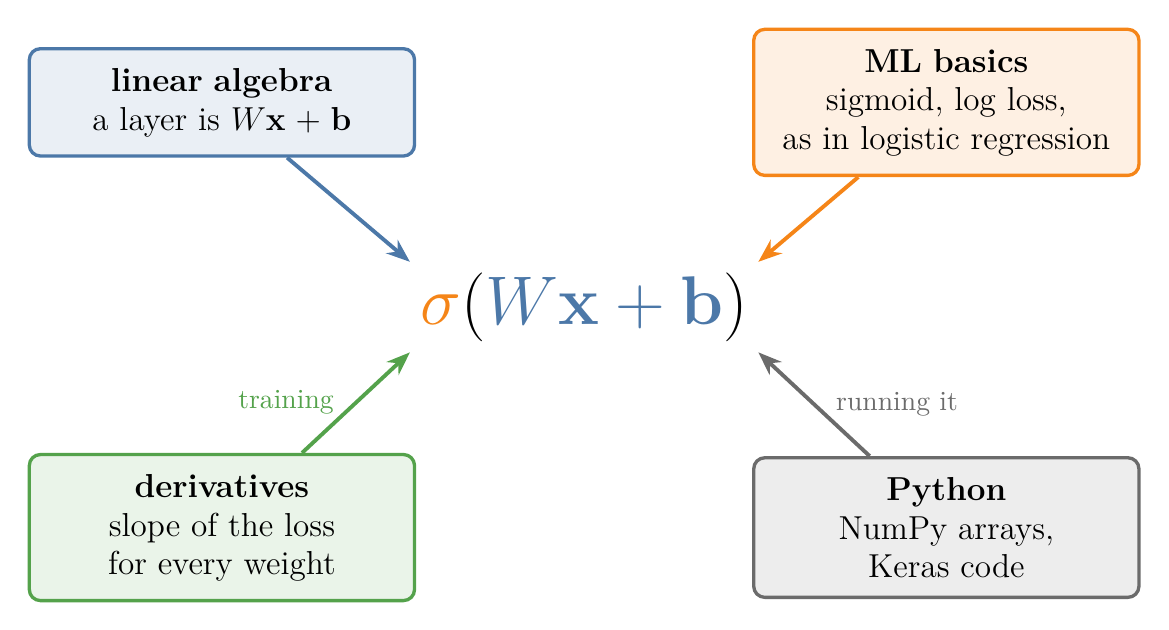
\begin{tikzpicture}[every node/.append style={font=\sffamily\large}]
  \node[font=\fontsize{30}{34}\selectfont] (f) at (0,0)
    {$\textcolor{corange}{\sigma}\big(\textcolor{cblue}{W\mathbf{x}+\mathbf{b}}\big)$};
  \node[box=cblue, text width=4.4cm] (la) at (-4.6,2.6) {\textbf{linear algebra}\\a layer is $W\mathbf{x}+\mathbf{b}$};
  \node[box=corange, text width=4.4cm] (ml) at (4.6,2.6) {\textbf{ML basics}\\sigmoid, log loss,\\as in logistic regression};
  \node[box=cgreen, text width=4.4cm] (de) at (-4.6,-2.8) {\textbf{derivatives}\\slope of the loss\\for every weight};
  \node[box=cgrey, text width=4.4cm] (py) at (4.6,-2.8) {\textbf{Python}\\NumPy arrays,\\Keras code};
  \draw[arrow, draw=cblue] (la) -- (f.north west);
  \draw[arrow, draw=corange] (ml) -- (f.north east);
  \draw[arrow, draw=cgreen] (de) -- node[left=4pt, text=cgreen, font=\sffamily] {training} (f.south west);
  \draw[arrow] (py) -- node[right=4pt, text=cgrey, font=\sffamily] {running it} (f.south east);
\end{tikzpicture}
\end{document}
